\section{结果与评价}
\subsection{实验设置}
\subsubsection{实验环境与数据划分}
本文全部实验在单张 NVIDIA GeForce RTX 5090（32 GB 显存）上完成，软件环境为 Linux 操作系统、Python 3.11 与 PyTorch 2.12（CUDA 13.0）。

实验数据取自 \texttt{im2latex-100k} 数据集：从其训练划分中选取 $50{,}000$ 个样本，
并以固定随机种子（$\texttt{SPLIT\_SEED}=42$）随机划分为 $40{,}000$ 个训练样本与 $10{,}000$ 个验证样本；
测试集取自该数据集独立的测试划分，共 $2{,}000$ 个样本。
采用固定种子的随机划分而非按顺序截取末尾样本，是为了避免数据集内部可能存在的排序偏置
（如按公式长度排序）导致验证集分布失真，同时保证数据划分可复现（训练过程的权重初始化、Dropout 与批次打乱未设全局种子，不同次训练的结果未必逐位一致，参见后文训练稳定性分析）。
基于训练语料构建的词表共含 $504$ 个词元（含填充符与 \texttt{[UNK]}），
其边际熵为 $3.83$，显著低于均匀分布熵 $\ln 504 \approx 6.22$，
表明 LaTeX 词元分布高度不均衡，这也是输出层引入词频先验偏置的依据。

\subsubsection{超参数配置}
模型与训练的完整超参数配置如表~\ref{tab:hyperparams} 所示。
模型总参数量为 $7.73$M，其中 ViT 编码器 $4.27$M、解码器（含嵌入与输出层）$3.46$M，
属轻量级配置。

\begin{table}[htbp]
    \centering
    \caption{模型与训练超参数配置}
    \begin{tabular}{llll}
        \toprule
        \textbf{类别} & \textbf{超参数} & \textbf{取值} & \textbf{说明} \\
        \midrule
        \multirow{4}{*}{输入}
        & 图像尺寸 & $50 \times 200 \times 1$ & 灰度图，像素归一化至 $[0,1]$ \\
        & 图像块大小 & $10 \times 10$ & 共 $100$ 个图像块 \\
        & 词表大小 & $504$ & 含填充符与 \texttt{[UNK]} \\
        & 最大序列长度 & $152$ & 含 \texttt{[START]}/\texttt{[END]} \\
        \midrule
        \multirow{3}{*}{编码器}
        & 层数 / 注意力头数 & $8$ / $4$ & 每头维度 $256/4=64$ \\
        & 嵌入维度 & $256$ & — \\
        & MLP 隐藏维度 & $[512, 256]$ & GELU 激活 \\
        \midrule
        \multirow{2}{*}{解码器}
        & 层数 / 注意力头数 & $4$ / $8$ & 每头维度 $256/8=32$ \\
        & 前馈网络维度 & $512 \to 256$ & ReLU 激活 \\
        \midrule
        \multirow{6}{*}{训练}
        & 批大小 & $768$ & 每轮约 $52$ 个优化步 \\
        & 优化器 & AdamW & $\beta_1{=}0.9$，$\beta_2{=}0.98$，$\epsilon{=}10^{-9}$ \\
        & 权重衰减 & $10^{-4}$ & 解耦式权重衰减 \\
        & 学习率调度 & 预热 $800$ 步 & 峰值约 $2.2\times10^{-3}$ \\
        & 梯度裁剪 & 全局范数 $1.0$ & 防止训练发散 \\
        & Dropout / 早停 & $0.1$ / patience $10$ & 监控验证损失 \\
        \bottomrule
    \end{tabular}
    \label{tab:hyperparams}
\end{table}

\subsection{训练过程与稳定性分析}
\subsubsection{收敛过程}
图~\ref{fig:training-history} 给出了训练与验证集上掩蔽损失和掩蔽准确率随训练轮次的变化曲线。
训练在第 $78$ 轮由早停机制终止：验证损失在第 $68$ 轮达到最优值 $0.4427$（对应验证准确率 $90.5\%$），
其后连续 $10$ 轮未再改善，训练终止并自动回退至最优轮次的权重。
整个训练过程损失单调平稳下降，未出现震荡或发散；
训练与验证曲线在前 $25$ 轮几乎重合，其后训练损失继续下降而验证损失趋于平台（最终训练损失 $0.105$、验证损失约 $0.45$），
呈现轻度而可控的过拟合，早停机制有效阻止了其进一步扩大。

\begin{figure}[H]
    \centering
    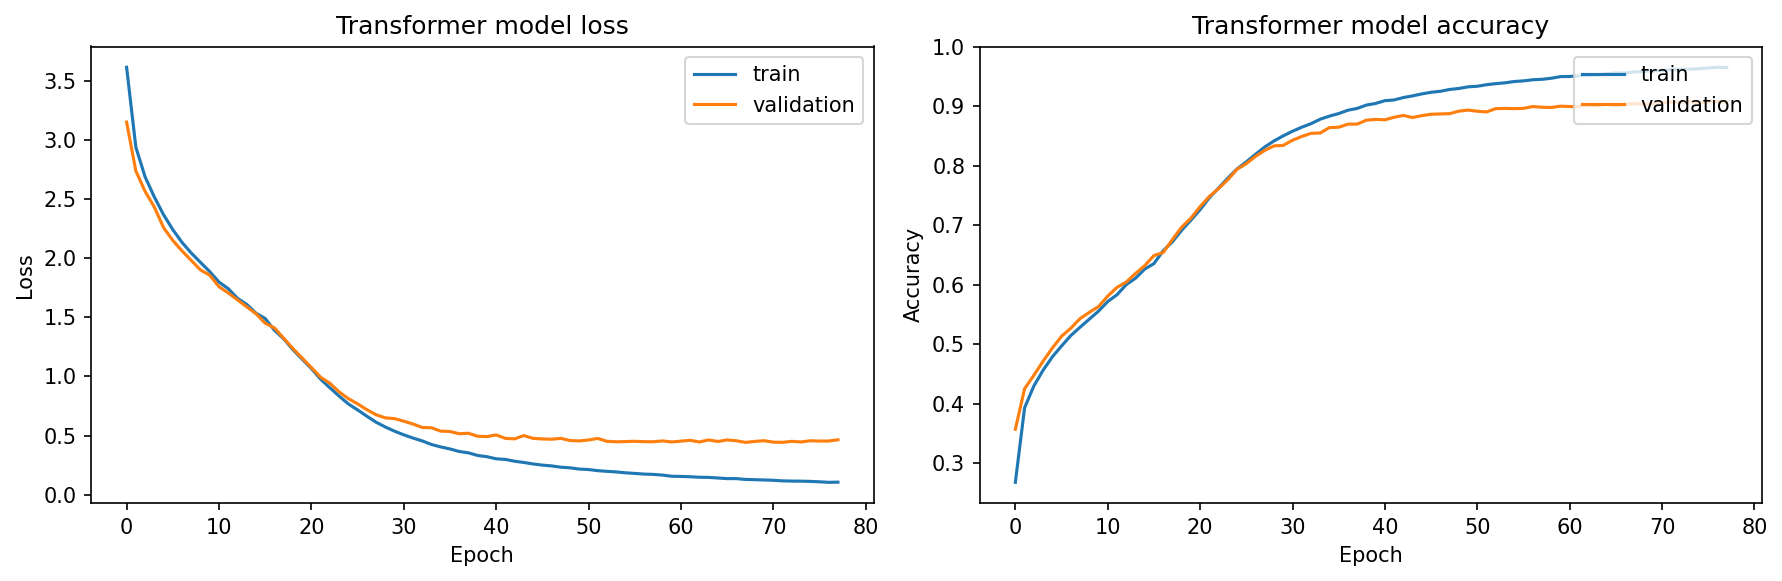
\includegraphics[width=\textwidth]{pic/training_history}
    \caption{训练与验证集上的掩蔽损失（左）与掩蔽准确率（右）变化曲线}
    \label{fig:training-history}
\end{figure}

\subsubsection{训练稳定性与梯度裁剪的必要性}
在大批量（$768$）配合预热调度的设定下，本文实验观察到了显著的训练稳定性问题，
为梯度裁剪的必要性提供了直接的实验证据：

\begin{enumerate}[label={（\arabic*）}, leftmargin=2em, labelsep=0.5em, itemsep=0pt]
    \item {无梯度裁剪时训练对随机性高度敏感}：在预热步数为 $500$（峰值学习率约 $2.8\times10^{-3}$）、
    无梯度裁剪的配置下，两次仅随机种子不同的训练呈现截然不同的结局——
    一次正常收敛，另一次在第 $7$ 轮（恰处于学习率爬升至峰值附近的阶段）突然发散：
    损失由 $2.07$ 跳升至 $4.02$，此后模型坍缩为退化解，
    无论输入何种图像均重复输出最高频词元 \texttt{\{} 与 \texttt{\}}，
    掩蔽准确率恰好卡死在该类词元的边际频率（约 $16.4\%$）附近，且无法依靠后续训练自行恢复；
    \item {发散机理}：预热阶段后期学习率接近峰值，此时单个梯度范数异常的批次即可在一步更新中
    将权重推离正常区域；模型一旦落入“仅输出高频词元”的退化局部极小，
    其梯度信号近乎平坦，以衰减后的学习率难以逃逸；
    \item {修复措施及效果}：引入全局范数为 $1.0$ 的梯度裁剪，并将预热步数提高至 $800$
    （峰值学习率降至约 $2.2\times10^{-3}$）后，训练全程（$78$ 轮、约 $4{,}100$ 个优化步）
    未再出现任何失稳迹象；在本次对比中，其最终验证损失亦略低于此前无裁剪的成功训练
    （$0.4427$ 对 $0.4628$；两次训练的预热步数不同，此处仅作参考）。
\end{enumerate}

该现象与 Transformer 训练的已有经验一致：在大批量、强预热的设定下，
梯度裁剪并非可选的保守措施，而是保证训练可靠完成的必要组件。

\subsection{主要结果}
模型在独立测试集（$2{,}000$ 个样本）上的总体性能如表~\ref{tab:results} 所示。
其中掩蔽损失与掩蔽准确率在教师强制（teacher forcing）模式下逐词元计算（按批次求均值后再对批次取平均）；
BLEU-4 分数则在完全自回归生成模式下计算（对 $500$ 个测试样本解码，
采用 method1 平滑），更真实地反映模型实际推理时的生成质量。

\begin{table}[H]
    \centering
    \caption{模型在 \texttt{im2latex-100k} 测试集上的总体性能}
    \begin{tabular}{lcc}
        \toprule
        \textbf{指标} & \textbf{评估模式} & \textbf{数值} \\
        \midrule
        掩蔽损失（Masked Loss） & 教师强制 & $0.4551$ \\
        掩蔽准确率（Masked Accuracy） & 教师强制 & $90.14\%$ \\
        BLEU-4（贪婪解码） & 自回归生成 & $0.6767$ \\
        BLEU-4（束搜索，$k=4$） & 自回归生成 & $\mathbf{0.7012}$ \\
        \bottomrule
    \end{tabular}
    \label{tab:results}
\end{table}

对上述结果作如下分析：
\begin{enumerate}[label={（\arabic*）}, leftmargin=2em, labelsep=0.5em, itemsep=0pt]
    \item {泛化一致性}：测试集掩蔽损失（$0.4551$）与验证集最优损失（$0.4427$）十分接近，
    测试准确率（$90.14\%$）与验证准确率（$90.5\%$）基本持平，
    表明模型未对验证集产生选择性过拟合，所报告的性能具有可靠的泛化意义；
    \item {教师强制指标与生成指标的差距}：教师强制下逐词元准确率达 $90.14\%$，
    而自回归生成的 BLEU-4 为 $0.68 \sim 0.70$。二者的差距源于自回归解码的误差累积效应——
    教师强制模式下每一步均以真实历史为条件，而实际生成中早期的词元错误会改变后续所有预测的条件分布。
    这一差距也印证了仅以教师强制准确率评估生成模型会系统性高估其实际能力，
    自回归 BLEU 才是更接近真实使用场景的指标；
    \item {与代表性方法的关系}：在相同数据集上，以全分辨率图像和更大模型容量为代价的专用方法
    （如基于由粗到细注意力的模型\supercite{dengImagetomarkupGenerationCoarsetofine2017}）
    报告了更强的识别性能；需说明的是，其评测协议（分词方式、平滑策略与样本规模）与本文不完全一致，相关数值不宜直接逐位比较。本文模型以 $50\times200$ 的低分辨率输入与 $7.73$M 的轻量参数规模
    取得约 $0.70$ 的 BLEU-4，在该量级的轻量配置下验证了纯 Transformer 架构在该任务上的有效性；
    分辨率与模型容量带来的性能上限将在第~\ref{subsec:limitations} 节进一步讨论。
\end{enumerate}

\subsection{解码策略对比}
为考察解码策略对生成质量的影响，在同一组 $500$ 个测试样本上分别采用贪婪解码与束搜索解码
（束宽 $k=4$，GNMT 长度惩罚\supercite{wuGoogleNeuralMachine2016} $\alpha=0.6$）\supercite{vaswaniAttentionAllYou2017}，结果如表~\ref{tab:decoding} 所示。

\begin{table}[H]
    \centering
    \caption{贪婪解码与束搜索解码的 BLEU-4 对比（同一组 500 个测试样本）}
    \begin{tabular}{lccc}
        \toprule
        \textbf{解码策略} & \textbf{BLEU-4} & \textbf{绝对提升} & \textbf{相对提升} \\
        \midrule
        贪婪解码 & $0.6767$ & — & — \\
        束搜索（$k=4$，$\alpha=0.6$） & $\mathbf{0.7012}$ & $+0.0245$ & $+3.6\%$ \\
        \bottomrule
    \end{tabular}
    \label{tab:decoding}
\end{table}

在该 $500$ 样本测试集上，束搜索带来 $2.45$ 个 BLEU 点的提升，处于序列生成任务中束搜索的典型收益区间（$1\sim3$ 点）。
其改进来源于两方面：其一，贪婪解码在每步只保留局部最优词元，
而 LaTeX 语法中大量结构性词元（如 \texttt{\{}、\texttt{\textasciicircum}、\texttt{\_}）的正确选择
往往依赖于其后若干步的整体合理性，束搜索通过并行维护多条候选序列缓解了这种局部最优陷阱；
其二，GNMT 长度惩罚对累计对数概率按长度归一化，抑制了概率连乘天然偏好短序列的系统性偏差，
减少了生成结果的过早截断。其代价是推理时每步需对至多 $k$ 条候选并行前向计算，
推理开销约为贪婪解码的 $3 \sim 4$ 倍，属于典型的“以计算换质量”的权衡。

\subsection{手写场景对比实验}
\label{subsec:handwriting}
为考察上述方法向手写场景迁移的能力，本文在手写体数据集 \texttt{MathWriting-human} 上
以\textbf{完全相同}的模型架构与训练配方（$50{,}000$ 个训练样本、批大小 $768$、
预热 $800$ 步、梯度裁剪 $1.0$、早停 patience $10$）开展对比实验。
该数据集的公式为未分词的原始 LaTeX 字符串，经正则词元化后构建词表，
共 $235$ 个词元（边际熵 $3.69$，均匀分布熵 $\ln 235 \approx 5.46$），
显著小于印刷体数据集的词表（$504$）——手写采集场景下的公式整体更短、符号集更集中。
测试集取自该数据集独立的测试划分（$2{,}000$ 个样本）。

\subsubsection{训练过程与双数据集结果对比}
图~\ref{fig:training-history-mathwriting} 给出了手写体实验的训练曲线：
训练于第 $33$ 轮早停，验证损失在第 $23$ 轮达到最优值 $0.9215$（验证准确率约 $79\%$）。
与印刷体实验（图~\ref{fig:training-history}）相比，过拟合显著提前且幅度更大——
早停时训练损失已降至 $0.34$ 而验证损失停滞在 $0.92$ 附近，
表明在书写风格高度多样的手写数据上，$50{,}000$ 个样本不足以支撑模型泛化。
值得注意的是，训练全程依然平稳无发散，说明梯度裁剪与预热调度构成的训练配方
对数据分布的变化具有良好的鲁棒性。

\begin{figure}[H]
    \centering
    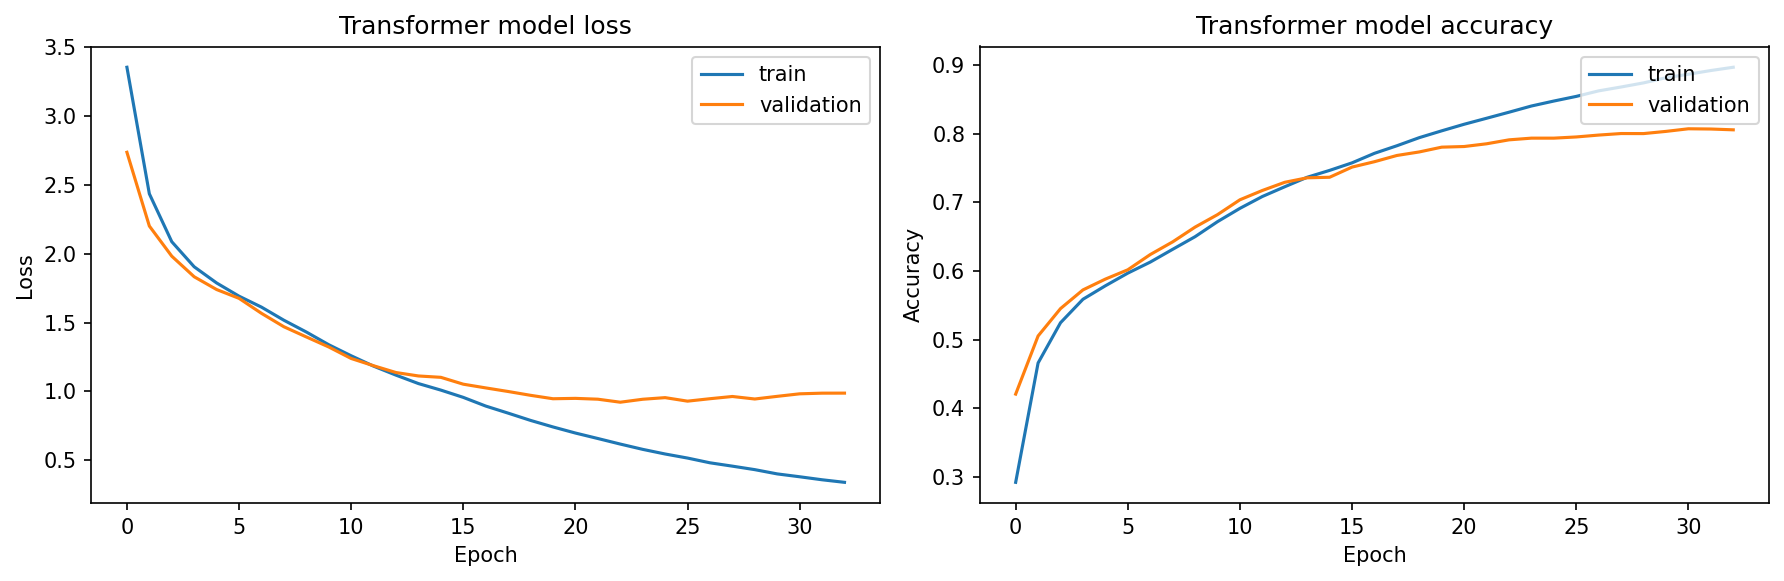
\includegraphics[width=\textwidth]{pic/training_history_mathwriting}
    \caption{\texttt{MathWriting-human} 上的训练曲线：验证损失于第 23 轮触底后走平，
    训练损失持续下降，呈现明显过拟合}
    \label{fig:training-history-mathwriting}
\end{figure}

两个数据集上的完整结果对比如表~\ref{tab:dataset-comparison} 所示。

\begin{table}[H]
    \centering
    \caption{印刷体与手写体数据集上的性能对比（相同架构与训练配方）}
    \begin{tabular}{lcc}
        \toprule
        \textbf{指标} & \texttt{im2latex-100k}（印刷体） & \texttt{MathWriting-human}（手写体） \\
        \midrule
        词表大小 & $504$ & $235$ \\
        训练轮数（早停） & $78$ & $33$ \\
        最优验证损失 & $0.4427$ & $0.9215$ \\
        最优验证掩蔽准确率 & $90.5\%$ & $\approx 79\%$ \\
        测试损失 & $0.4551$ & $2.1402$ \\
        测试掩蔽准确率 & $90.14\%$ & $56.63\%$ \\
        BLEU-4（贪婪解码） & $0.6767$ & $0.0833$ \\
        BLEU-4（束搜索，$k=4$） & $0.7012$ & $0.0786$ \\
        \bottomrule
    \end{tabular}
    \label{tab:dataset-comparison}
\end{table}

\subsubsection{性能差距的成因分析}
手写体上的性能大幅下降并非单一因素所致：以下前三点为模型与数据层面、可分别施治的成因，第四点则为评测指标对短序列的放大效应（属测量层面，而非模型本身缺陷），具体如下：
\begin{enumerate}[label={（\arabic*）}, leftmargin=2em, labelsep=0.5em, itemsep=0pt]
    \item {书写者分布偏移（最主要因素）}：验证集与训练集取自同一批样本的随机划分，
    二者共享书写者与书写风格，故验证准确率高达约 $79\%$；
    而测试划分来自独立的数据来源，测试准确率骤降至 $56.63\%$（测试损失 $2.14$ 对验证 $0.92$）。
    这一验证--测试鸿沟在印刷体实验中几乎不存在（$0.4427$ 对 $0.4551$），
    定量刻画了手写识别特有的跨书写者泛化难题；
    \item {样本量不足导致的过拟合}：印刷体的视觉模式高度标准化，$50{,}000$ 个样本已足够；
    手写体的同一符号在不同书写者笔下差异巨大，相同样本量下模型转而记忆训练样本的个体特征，
    训练曲线的提前分化即为直接证据。本实验为保证与印刷体严格可比而未使用
    \texttt{MathWriting-human} 的全部约 $230{,}000$ 个训练样本，也未引入任何数据增强；
    \item {几何失真}：手写采集图像的宽高比接近 $1{:}1.3$（如 $187\times141$），
    被强制缩放至 $50\times200$（宽高比 $4{:}1$）时产生严重的横向拉伸，
    笔画形态信息损失远大于本身即为宽幅排版的印刷体公式图像；
    \item {BLEU 对短参考序列的敏感性}：手写数据集的公式整体较短（不少参考序列不足 $10$ 个词元），
    BLEU-4 的高阶 $n$-gram 在短序列上极易失配，对相同的词元级错误率给出远低于长序列的分数，
    放大了两个数据集间生成指标的表观差距。
\end{enumerate}

此外，束搜索在手写体上未带来增益（$0.0786$ 对 $0.0833$）。
这与解码理论的预期一致：束搜索的收益建立在模型条件分布校准良好的前提上，
当模型本身欠拟合目标分布时，搜索更宽只会更彻底地利用一个不可靠的概率模型，
长度惩罚在大量短序列上的归一化也会进一步引入偏差。
该结果亦与表~\ref{tab:decoding} 的印刷体实验相呼应：束搜索的增益依赖于模型条件分布的校准质量，而非搜索算法本身；但二者序列长度分布差异较大，此处仅作定性参照。

定性考察（图~\ref{fig:predictions-mathwriting}）与上述分析吻合：
模型生成的序列几乎全部语法合法——分式、上下标乃至括号内的矩阵结构均能正确组织，
说明解码器习得的 LaTeX 语法先验迁移良好；笔迹清晰、结构简单的样本亦能被完整正确识别
（如图~\ref{fig:predictions-mathwriting} 左上样本所示的积分关系式 $\int \mathrm{d}V\,|\Psi|^{2}=N$ 被逐词元准确还原）。
但生成内容与图像的对应关系明显弱于印刷体，最典型的是“结构正确但符号识别有误”的输出——
例如图~\ref{fig:predictions-mathwriting} 右上样本正确还原了括号内的二行矩阵结构，
却把分子 $2r-1$ 误识为 $n+1$；表明主要瓶颈在于模型对手写笔迹的视觉特征提取与跨模态对齐，
而非语言建模能力。

\begin{figure}[H]
    \centering
    
\includegraphics[width=\textwidth]{pic/predictions_mathwriting}
    \caption{\texttt{MathWriting-human} 测试样本的预测结果与真实标签对照（左上为正确识别，右上为结构正确但符号识别有误，下方两例为错误识别）}
    \label{fig:predictions-mathwriting}
\end{figure}

\subsection{定性分析与误差分析}
本节针对印刷体（\texttt{im2latex-100k}）实验的生成结果展开定性与误差分析。
\subsubsection{生成质量的定性考察}
图~\ref{fig:predictions} 展示了测试集样本的预测结果与真实标签对照。
对测试集随机样本的人工考察表明，模型生成的 LaTeX 序列绝大多数语法完整、花括号正确配对，
能够直接通过 LaTeX 编译。模型对多种复杂结构均能正确建模，包括：
嵌套分式与根式（如 $\texttt{\textbackslash sqrt\{\textbackslash frac\{...\}\{...\}\}}$）、
多重上下标与张量指标链、求和与积分的上下限结构、
函数算符（\texttt{\textbackslash operatorname\{sin\}}、$\texttt{\textbackslash operatorname*\{lim\}}$）乃至
\texttt{\textbackslash begin\{array\}} 环境下的矩阵与行列式
（如图~\ref{fig:demo-samples}（b）所示的 $2\times2$ 分块行列式，其 \texttt{array} 主体结构被正确还原，仅末项的行列式定界符 $\lvert\cdot\rvert$ 被误生成为方括号）。

\begin{figure}[H]
    \centering
    
\includegraphics[width=\textwidth]{pic/predictions}
    \caption{测试集样本的预测结果（Predicted）与真实标签（Ground truth）对照}
    \label{fig:predictions}
\end{figure}

\begin{figure}[H]
    \centering
    \begin{subfigure}[b]{0.48\textwidth}
        \centering
        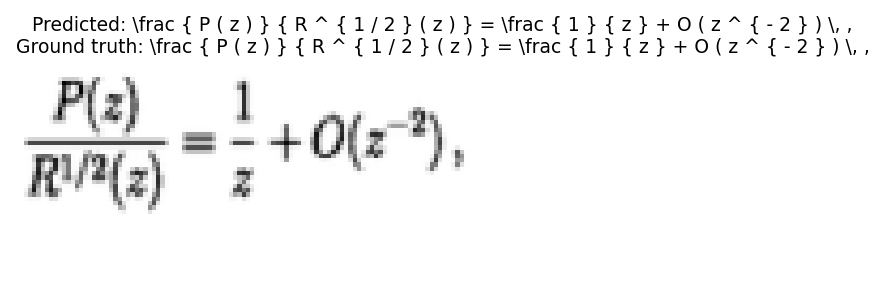
\includegraphics[width=\linewidth]{pic/demo_simple_sample}
        \caption{含渐近 $O$ 记号的分式表达式}
        \label{fig:demo-simple}
    \end{subfigure}
    \hfill
    \begin{subfigure}[b]{0.48\textwidth}
        \centering
        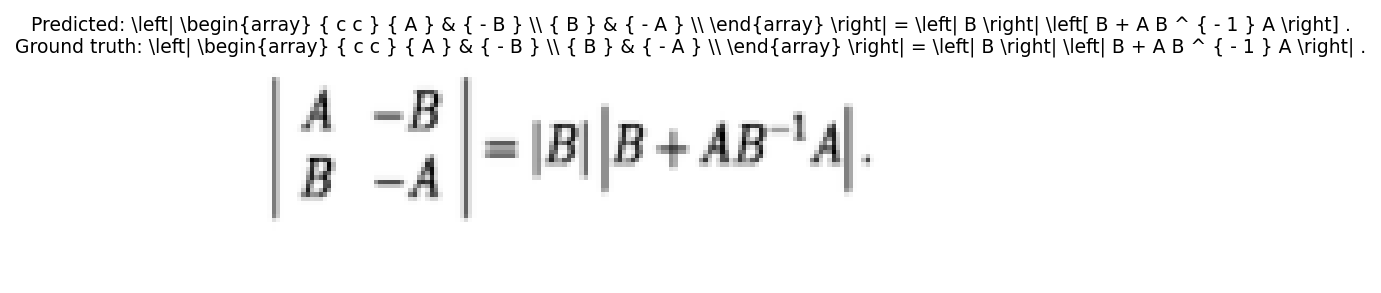
\includegraphics[width=\linewidth]{pic/demo_array_sample}
        \caption{含 \texttt{array} 环境的分块行列式}
        \label{fig:demo-array}
    \end{subfigure}
    \caption{随机测试样本的生成结果示例}
    \label{fig:demo-samples}
\end{figure}

\subsubsection{典型错误模式}
对生成失败的样本进行归类，主要错误模式及其成因如下：
\begin{enumerate}[label={（\arabic*）}, leftmargin=2em, labelsep=0.5em, itemsep=0pt]
    \item {相似符号混淆}：低分辨率输入（$50\times200$）下视觉上相近的符号易被混淆，
    如上下标位置的数字与字母、$\texttt{\textbackslash partial}$ 与 $\partial$ 形近符号等。
    此类错误为单词元替换，对 BLEU 的高阶 $n$-gram 影响有限但直接影响语义正确性；
    \item {长序列后段退化}：在较长表达式的生成后段偶见词元序列退化
    （如下标中字母被逐个拆散为无意义组合），
    反映了自回归解码误差累积与低分辨率下细节信息不足的叠加效应；
    \item {括号失配残留}：极少数样本存在多余或缺失的右花括号或
    \texttt{\textbackslash left}/\texttt{\textbackslash right} 定界符失配，
    导致编译失败。该类错误源于模型缺乏对括号配对的显式约束，
    完全依赖数据驱动的隐式学习；
    \item {词表外词元不可生成}：词表基于 $50{,}000$ 个训练样本构建（$504$ 个词元），
    测试集中出现的词表外（OOV）词元被映射为 \texttt{[UNK]}，而 \texttt{[UNK]} 在输出层被先验偏置禁止生成，
    故含罕见命令的表达式必然无法完整复原。
    评估时此类位置已通过掩蔽机制从损失统计中排除，但其对 BLEU 的影响真实存在。
\end{enumerate}

\subsection{局限性与展望}
\label{subsec:limitations}
本文工作的主要局限与相应的改进方向如下：
\begin{enumerate}[label={（\arabic*）}, leftmargin=2em, labelsep=0.5em, itemsep=0pt]
    \item {输入分辨率}：$50\times200$ 的输入尺寸对长公式压缩严重，
    是相似符号混淆与细节丢失的首要原因。提高输入分辨率（并相应增大图像块数量）
    是性能提升空间最明确的方向，其代价是自注意力计算量随图像块数二次增长；
    \item {模型容量}：$7.73$M 的参数规模远小于该任务的专用模型，
    在训练数据充足的前提下，加深加宽模型有望进一步缩小与专用方法的差距；
    \item {解码约束}：当前解码过程无语法约束，括号失配等结构性错误只能依靠数据隐式纠正。
    引入语法感知的约束解码或树结构解码器\supercite{zhuTAMERTreeawareTransformer2024}
    是改善结构正确性的可行途径；
    \item {手写场景的针对性改进}：第~\ref{subsec:handwriting} 节的对比实验定量揭示了
    直接迁移印刷体配方的三个瓶颈，对应的改进方向均有明确依据：
    针对跨书写者泛化与过拟合，应使用 \texttt{MathWriting-human} 的全部约 $230{,}000$
    个训练样本并配合数据增强（随机仿射变换、弹性形变）；
    针对几何失真，应采用保持宽高比的缩放加填充策略替代直接拉伸；
    在此基础上再叠加更高输入分辨率，预期可显著缩小手写与印刷体之间的性能差距。
\end{enumerate}

综上，本文构建的 ViT 编码器--Transformer 解码器模型在印刷体数据集 \texttt{im2latex-100k} 上
取得了 $90.14\%$ 的词元级准确率与 $0.7012$ 的 BLEU-4 分数（束搜索解码），
以轻量的模型规模与低分辨率输入验证了纯 Transformer 架构在数学表达式识别与 LaTeX
转换任务上的有效性；训练稳定性分析为大批量预热调度下梯度裁剪的必要性提供了直接的实验证据；
手写体对比实验则在严格控制变量的前提下，将手写场景的难度定量分解为
书写者分布偏移、样本量不足与几何失真三个可分别施治的因素，为后续改进指明了路径。
